\section{Inference Queries}
We have seen two major types of compact representations of joint probability distributions in terms of graphs. Summarizing the expressions of the joint distribution, we can write
\begin{align}
\text{For UGM: }\Prob(x_1, \cdots, x_n) &= \dfrac{1}{Z}\prod_C \psi_C(x_C) \\
\text{For DGM: }\Prob(x_1, \cdots, x_n) &= \prod_i \Prob(x_i|\text{Pa}(x_i))
\end{align}
We get a very compact representation if $\text{Pa}(x_i)$ is small. \\
Given a probability distribution $P$, we can ask two major types of queries - 
\begin{enumerate}
	\item \textit{Marginal probability queries over a sm`all subset of variables: }Given $P$, what is the marginal probability of $x_1$?.
	\begin{equation}
	\begin{split}
		\Prob(x_1) &= \sum_{x_2, \cdots, x_n} \Prob(x_1, \cdots, x_n) \\
		&= \sum_{x_2=1}^m \cdots \sum_{x_n=1}^m \Prob(x_1, \cdots, x_n)
	\end{split}
	\end{equation}
We can see that if each variable takes $m$ values, then the brute-force computation of the marginal probability will take $\mathcal{O}(m^{n-1})$ time.
\item \textit{Most likely labels of remaining variables (MAP queries): }Here, we ask questions of the form,
\begin{equation}
	\mathbf{x}^* = \argmax_{x_1, \cdots, x_n} \Prob(x_1, \cdots, x_n)
\end{equation}
An example of such a query could be - find the most likely entity labels of all words in a sentence.
\end{enumerate}
\begin{exmp}[Exact Inference]
Say we have a probability distribution over three binary variables as 
\[P(x_1, x_2, x_3) = \dfrac{1}{Z}\psi_{12}(x_1, x_2)\psi_{23}(x_2, x_3)\]
\begin{marginfigure}
	\centering
	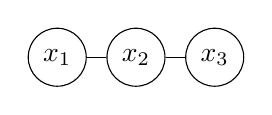
\begin{tikzpicture}[main/.style = {draw, circle}] 
		\node[main] (1) {$x_1$}; 
		\node[main] (2) [right of=1] {$x_2$}; 
		\node[main] (3) [right of=2] {$x_3$}; 
		\draw[-] (1) -- (2);
		\draw[-] (2) -- (3);
	\end{tikzpicture}
	\caption{UGM for $P(x_1, x_2, x_3)$}
	\label{fig:iq-p123-ugm}		
\end{marginfigure}
The UGM for this is shown in Figure \ref{fig:iq-p123-ugm}. Say we have the potential tables (each entry being $\psi_{ij}(a,b)$ representing the potential) as
\begin{center}
	\begin{tabular}{cc|c|c|}
		& \multicolumn{1}{c}{} & \multicolumn{2}{c}{$x_2$}\\
		& \multicolumn{1}{c}{} & \multicolumn{1}{c}{$0$}  & \multicolumn{1}{c}{$1$} \\\cline{3-4}
		\multirow{2}*{$x_1$}  & $0$ & $5$ & $2	$ \\\cline{3-4}
		& $1$ & $1$ & $4$ \\\cline{3-4}
	\end{tabular}
\qquad
\begin{tabular}{cc|c|c|}
	& \multicolumn{1}{c}{} & \multicolumn{2}{c}{$x_3$}\\
	& \multicolumn{1}{c}{} & \multicolumn{1}{c}{$0$}  & \multicolumn{1}{c}{$1$} \\\cline{3-4}
	\multirow{2}*{$x_2$}  & $0$ & $2$ & $10$ \\\cline{3-4}
	& $1$ & $5$ & $3$ \\\cline{3-4}
\end{tabular}
\end{center}
For example, we see that $\psi_{12}(0,0) = 5$. Let us find $P(x_1)$. 
\[P(x_1) =\dfrac{1}{Z} \sum_{x_2 \in \{0,1\}}\sum_{x_3 \in \{0,1\}}\psi_{12}(x_1, x_2)\psi_{23}(x_2, x_3)\]
We multiply the above two tables to get an intermediate potential distribution $\psi_{123}(x_1, x_2, x_3)$ and get a three dimensional table as follows (note that the columns denote $x_2$ and the rows denote $x_1$)
\begin{center}
	\begin{tabular}{cc|c|c|}
		& \multicolumn{1}{c}{} & \multicolumn{2}{c}{$x_3=0$}\\
		& \multicolumn{1}{c}{} & \multicolumn{1}{c}{$0$}  & \multicolumn{1}{c}{$1$} \\\cline{3-4}
		\multirow{2}*{}  & $0$ & $10$ & $10	$ \\\cline{3-4}
		& $1$ & $2$ & $20$ \\\cline{3-4}
	\end{tabular}
	\qquad
	\begin{tabular}{cc|c|c|}
		& \multicolumn{1}{c}{} & \multicolumn{2}{c}{$x_3=1$}\\
		& \multicolumn{1}{c}{} & \multicolumn{1}{c}{$0$}  & \multicolumn{1}{c}{$1$} \\\cline{3-4}
		\multirow{2}*{}  & $0$ & $50$ & $6$ \\\cline{3-4}
		& $1$ & $10$ & $12$ \\\cline{3-4}
	\end{tabular}
\end{center}
For example, $\psi_{12}(0,0)\psi_{23}(0,0) = 2\times5=10$. The next computation is to sum over $x_3$.
\[P(x_1) = \dfrac{1}{Z} \sum_{x_2 \in \{0,1\}} \psi_{12}^*(x_1, x_2)\]
The table after sum denoting $\psi_{12}^*(x_1, x_2)$ is
\begin{center}
	\begin{tabular}{cc|c|c|}
		& \multicolumn{1}{c}{} & \multicolumn{2}{c}{$x_2$}\\
		& \multicolumn{1}{c}{} & \multicolumn{1}{c}{$0$}  & \multicolumn{1}{c}{$1$} \\\cline{3-4}
		\multirow{2}*{$x_1$}  & $0$ & $60$ & $16$ \\\cline{3-4}
		& $1$ & $12$ & $32$ \\\cline{3-4}
	\end{tabular}
\end{center}
Now we eliminate $x_2$ by summing over the row values, thus finally
\[
\psi_1^*(x_1) = \dfrac{1}{Z}\begin{bmatrix}
	76 \\ 44
\end{bmatrix}
\]
Since this $P(x_1) = \psi_1^*(x_1)$, we immediately get to know that $Z = 76+44 = 120$. \\
Clearly, we see through the example that the calculation, even for three variables is cumbersome. Image doing this for thousands! \\
From the table in the above example, we can also calculate the assignment which gives the maximum probability. Note the $\psi_{123}$ table made, and see that $x_1=0, x_2=0, x_3=1$ has the score of $50$ giving the highest probability. But let us write this in a more algorithmic way
\[\mathbf{x^*} = \argmax_{x_2} \argmax_{x_2}\argmax_{x_3} \psi_{12}(x_1,x_2)\psi_{23}(x_2,x_3) \]
Let us construct the table $\psi_{12}^{\max} (x_1, x_2)$ from the $\psi_{123}$ table
\begin{center}
	\begin{tabular}{cc|c|c|}
		& \multicolumn{1}{c}{} & \multicolumn{2}{c}{$x_2$}\\
		& \multicolumn{1}{c}{} & \multicolumn{1}{c}{$0$}  & \multicolumn{1}{c}{$1$} \\\cline{3-4}
		\multirow{2}*{$x_1$}  & $0$ & $50$ for $x_3=1$ & $10$ for $x_3=0$ \\\cline{3-4}
		& $1$ & $10$ for $x_3=0$ & $20$ for $x_3=0$ \\\cline{3-4}
	\end{tabular}
\end{center}
Similarly, $\psi_1^{\max} (x_1)$ will be
\[
\begin{bmatrix}
	50 \text{ for $x_2=0, x_3=1$} \\ 20 \text{ for $x_2=1, x_3=0$} 
\end{bmatrix}
\]
At last, we can do an argmax over $x_1$ to get the assignment $x_1=0, x_2=0,x_3=1$ for the score of $50$.
\end{exmp}
Clearly, after the example, it is clear that we want to avoid the exponential overhead that brute-force approach applies.
\subsection{Exact Inference on Chains}
Consider the chain show in Figure \ref{fig:iq-chain}.
\begin{marginfigure}
	\centering
	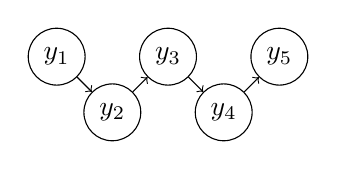
\begin{tikzpicture}[main/.style = {draw, circle}] 
		\node[main] (1) {$y_1$}; 
		\node[main] (2) [below right of=1] {$y_2$}; 
		\node[main] (3) [above right of=2] {$y_3$}; 
		\node[main] (4) [below right of=3] {$y_4$}; 
		\node[main] (5) [above right of=4] {$y_5$}; 
		\draw[->] (1) -- (2);
		\draw[->] (2) -- (3);
		\draw[->] (3) -- (4);
		\draw[->] (4) -- (5);
	\end{tikzpicture}
	\caption{Chain graph}
	\label{fig:iq-chain}		
\end{marginfigure}
We see that in the graph we would have potentials of the form $\psi_i(y_i, y_{i+1})$, and 
\begin{equation}
	\Prob(y_1, \cdots, y_n) = \prod_i \psi_i(y_i, y_{i+1})
\end{equation}
\textit{Note:} Since we don't have immoralities, the MRF is equivalent to the undirected version of the graph. Say we want to calculate 
\begin{equation}
\Prob(y_5=1) = \sum_{y_1, \cdots, y_4} \Prob(y_1, y_2, y_3, y_4, 1)
\end{equation}
The key idea to reducing computations is to push summations past the multiplications, i.e
\begin{equation}
\begin{split}
\Prob(y_5=1) &= \sum_{y_1, \cdots, y_4} \Prob(y_1, y_2, y_3, y_4, 1) \\
&= \sum_{y_1}\sum_{y_2}\sum_{y_3}\sum_{y_4} \psi_1(y_1, y_2)\psi_2(y_2,y_3)\psi_3(y_3,y_4)\psi_4(y_4,1) \\
&= \sum_{y_1}\sum_{y_2}\psi_1(y_1, y_2)\sum_{y_3}\psi_2(y_2, y_3)\sum_{y_4}\psi_3(y_3, y_4)\psi_4(y_4, 1) \\
&= \sum_{y_1}\sum_{y_2}\psi_1(y_1, y_2)\sum_{y_3}\psi_2(y_2, y_3)\mathcal{B}_3(y_3) \\
&= \sum_{y_1}\sum_{y_2}\psi_1(y_1, y_2) \mathcal{B}_2(y_2) \\
&= \sum_{y_1} \mathcal{B}_1(y_1) 
\end{split}
\end{equation}
We denote $\mathcal{B}_i(y_i)$ as the \textit{belief} which flows from node $i+1$ to $i$. This is an efficient computation. In general, if we have a chain with $n$ variables and each can take $m$ values, the above algorithm (breaking into beliefs) takes time in order of $\mathcal{O}(nm^2)$. \\
Notice that we did the efficient computation for chains, the natural question is, for what other graphs can this be done? \\
\begin{marginfigure}
	\centering
	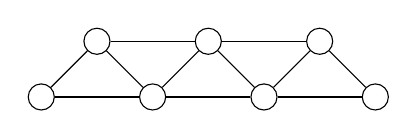
\begin{tikzpicture}[main/.style = {draw, circle}] 
		\node[main] (0) {};
		\node[main] (1) [above right of=0]{}; 
		\node[main] (2) [below right of=1] {}; 
		\node[main] (3) [above right of=2] {}; 
		\node[main] (4) [below right of=3] {}; 
		\node[main] (5) [above right of=4] {}; 
		\node[main] (6) [below right of=5] {}; 
		\draw[-] (0) -- (1);
		\draw[-] (1) -- (2);
		\draw[-] (0) -- (2);
		\draw[-] (1) -- (3);
		\draw[-] (2) -- (3);
		\draw[-] (2) -- (4);
		\draw[-] (3) -- (4);
		\draw[-] (3) -- (5);
		\draw[-] (4) -- (5);
		\draw[-] (4) -- (6);	
		\draw[-] (5) -- (6);
	\end{tikzpicture}
	\caption{Triangular graph}
	\label{fig:iq-triangle}		
\end{marginfigure}
Another one is shown in Figure \ref{fig:iq-triangle}. We define potential over each triangle (say $\psi_{123}$). If we follow a similar idea as the algorithm above, the time required for this computation will be $\mathcal{O}(nm^3)$.

\subsection{Hardness of Inference and 3-SAT}
The above discussion might lead to the thought that any graph $G$ which can be factorized into small clique sizes might have an efficient computation method (i.e polynomial time) of calculating the marginal probability.
\begin{marginfigure}
	\centering
	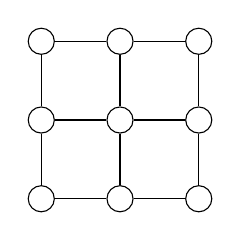
\begin{tikzpicture}[main/.style = {draw, circle}] 
		\node[main] (0) {};
		\node[main] (1) [right of=0]{}; 
		\node[main] (2) [right of=1] {}; 
		\node[main] (3) [below of=0] {}; 
		\node[main] (4) [below of=1] {}; 
		\node[main] (5) [below of=2] {}; 
		\node[main] (6) [below of=3] {}; 
		\node[main] (7) [below of=4] {}; 
		\node[main] (8) [below of=5] {}; 
		\draw[-] (0) -- (1);
		\draw[-] (1) -- (2);
		\draw[-] (0) -- (3);
		\draw[-] (1) -- (4);
		\draw[-] (2) -- (5);
		\draw[-] (3) -- (4);
		\draw[-] (5) -- (4);
		\draw[-] (3) -- (6);
		\draw[-] (4) -- (7);
		\draw[-] (5) -- (8);	
		\draw[-] (6) -- (7);
		\draw[-] (7) -- (8);
	\end{tikzpicture}
	\caption{Grid graph}
	\label{fig:iq-grid}		
\end{marginfigure}
 The answer sadly is no, and a counter example is the grid graph shown in Figure \ref{fig:iq-grid}. \\
 We will now reduce the $3$-SAT to inference in Bayesian Networks.
 \begin{defn}[$3$-SAT Problem]
 Given $n$ boolean variables $x_1, \cdots x_n$ such that $x_i \in \{T,F\}$. We define a literal $\ell$ to be the variable $x_i$ or its negation $\neg x_i$ or $\bar{x}_i$. Given a set of $K$ clauses $C_1, C_2, \cdots, C_K$ with each clause being
 \begin{equation} \label{eq:3-sat-clause}
 	C_j = \ell_{j_1} \lor \ell_{j_2} \lor \ell_{j_3}
 \end{equation}
The $3$-SAT problem is to decide if there exists an assignment of values to the $n$ variables such that 
\begin{equation}\label{eq:3-sat-sat}
	C_1 \land C_2 \land \cdots \land C_K = T
\end{equation}
 \end{defn}
\begin{exmp}\label{exmp:3-sat}
Consider $n=4, K=3$ and
\begin{align*}
	C_1 &= x_1 \lor \bar{x}_2 \lor \bar{x}_3 \\ 
	C_2 &= x_2 \lor x_3 \lor \bar{x}_4 \\
	C_3 &= x_4 \lor \bar{x}_1 \lor \bar{x}_2
\end{align*}
In this case, having all $x_i = T$ for $i = \{1, 2, 3, 4\}$ solves the problem.
\end{exmp}
In the above example, we by chance got lucky and solved the problem, but in general for a large number of variables, it is not possible to go over all possible combinations of values, since it requires an exponential amount of time. \\
Now we represent $3$-SAT as a Bayesian Network.
	\begin{marginfigure}
	\centering
	\begin{tikzpicture}[main/.style = {draw, circle}] 
		\node[main] (x1) {$x_1$}; 
		\node[main] (x2) [right of=x1] {$x_2$};
		\node[main] (x3) [right of=x2] {$x_3$};
		\node[main] (x4) [right of=x3] {$x_4$};
		\node[main] (c1) [below = of $(x1)!0.5!(x2)$] {$C_1$};
		\node[main] (c2) [below = of $(x2)!0.5!(x3)$] {$C_2$};
		\node[main] (c3) [below = of $(x3)!0.5!(x4)$] {$C_3$};
		\node[main] (s) [below = of c2] {$\mathcal S$};
     	\draw[->] (x1) -- (c1);
     	\draw[->] (x2) -- (c1);
     	\draw[->] (x3) -- (c1);
     	\draw[->] (x2) -- (c2);
     	\draw[->] (x3) -- (c2);
     	\draw[->] (x4) -- (c2);
     	\draw[->] (x4) -- (c3);
     	\draw[->] (x1) -- (c3);
     	\draw[->] (x2) -- (c3);
     	\draw[->] (c1) -- (s);
     	\draw[->] (c2) -- (s);
     	\draw[->] (c3) -- (s);
	\end{tikzpicture}
	\caption{3-SAT as BN}
	\label{fig:bn-3-sat}
\end{marginfigure}
Let us do that in a \textit{layer} sense. Let the first layer have all the variables as nodes and the next layer have all the clauses. Each clause will have 3 parents due to Equation \ref{eq:3-sat-clause}. Finally, the third layer would have $\mathcal S$, which is the satisfiability (Equation \ref{eq:3-sat-sat}), and it's parents would be all the clauses. Figure \ref{fig:bn-3-sat} shows the BN of Example \ref{exmp:3-sat}. \\
Coming back to the general setting, for each variable $x_i$, we denote
\begin{equation}
	\Prob(x_i) = \begin{cases}
		\frac{1}{2} & x_i=F \\
		\frac{1}{2} & x_i=T
	\end{cases}
\end{equation}

We also need to define $\Prob(C_j|\ell_{j_1}, \ell_{j_2}, \ell_{j_3})$. To do this, we assign a non-zero probability to only those which make $C_j=T$. This can be done uniformly (say out of the 8 assignments, 5 give a non-zero value, then $\frac{1}{5}$ for each of those assignments, and $0$ to rest). Finally, we write the last probability $\Prob(\mathcal S|C_1, \cdots, C_K)$ as $1$ if $C_1, \cdots, C_K = T$, i.e all are true, and in the rest of the cases, we assign it as zero (note the difference here - the table for each $C_i$ had 8 rows, and the table for $\mathcal S$ has $2^K$ rows). The $2^K$ shows that it is not polynomial. This is again, not efficient. \\
One small change we can do is that instead of having a single $\mathcal S$ in the last layer, have $K-1$, such that each $\mathcal{S}_i$ is connected to $C_{i-1}$ and $C_i$ as parents, and each $\mathcal{S}_i$ is a parent of $\mathcal{S}_{i+1}$. This allows us to create the probability table as $\Prob(\mathcal{S}_j | \mathcal{S}_{j-1}, C_{j-1}, C_j)$ which represents the logic
\begin{equation}
	\mathcal{S}_j =  \mathcal{S}_{j-1} \land C_{j-1} \land C_j 
\end{equation} 
This allows each $\mathcal{S}_j$ with 8 variables, bringing in the needed efficiency. \\
Finally, if we can answer $\Prob(\mathcal{S}_j=1) > 0$ positively, then we know that a $3$-SAT assignment exists, else it does not.